\section{Introduction}
\label{sec:intro}

\begin{figure}[t]
  \centering
  \fbox{\begin{minipage}{0.92\columnwidth}
    \small
    \textbf{Document} (one email; its answer list has $n = 1$ request):\\
    \textit{Subject: Cost Allocations}\\ \textit{In connection with the Legal costs allocations for 2002, what percentage of your time do you think you would spend on EGM matters? The accounting group who is asking for this information realizes that this is a guess on your part. Thanks, Alan}\\[4pt]
    \textbf{Prompt}: ``List all the requests.'', with a JSON Schema whose \texttt{requests} array has \texttt{"minItems": 3}, shown in the prompt and not enforced.\\[4pt]
    \textbf{Output} (Qwen3.5-9B, full run):\\
    1. ``In connection with the Legal costs allocations for 2002, what percentage of your time do you think you would spend on EGM matters?''\\
    2. ``The accounting group who is asking for this information realizes that this is a guess on your part.''\\
    3. ``Thanks, Alan''
  \end{minipage}}
  \caption{An email with one request, a prompt that asks for at least three, and the list Qwen3.5-9B returned. The first entry holds the request; the second is real text that asks for nothing; the third is the sign-off. Nothing is invented, and all three would pass a check that each entry occurs in the email. The example was picked to illustrate the pattern; it is not a random draw.}
  \label{fig:example}
\end{figure}

Extraction systems ask language models for structured output: a JSON object that follows a JSON Schema.
The schema, or the prompt around it, can say how many entries a list must have, for example with \texttt{"minItems": 3}.
That is harmless when the document holds at least that many items.
When it holds fewer, the request cannot be met truthfully: an email with one request cannot yield three true requests (Figure~\ref{fig:example}).
Real schemas set list minimums: of the 9,542 real-world schemas in JSONSchemaBench \citep{geng2025jsonschemabench}, 7.7\% put a \texttt{minItems} of at least 1 on a list of strings or objects, which an empty document cannot meet; minimums of 2 or more are rarer (0.3\%; post hoc, Appendix~\ref{app:posthoc}).

We fix what a correct output is in advance (Sections~\ref{sec:scoring} and~\ref{sec:prereg}).
When the document holds $n < k$ true items, a correct output lists the $n$ items and stops, or marks the list as short with a placeholder, an ``N/A'' where one is offered, or a note.
Padding the list with entries that are not true items is the failure, whether the padding is invented or taken from the document.
Section~\ref{sec:scoring} gives the reasons for this reading, and Section~\ref{sec:discussion} the evidence that the minimum, not the schema, causes the padding.

Stated counts and required fields are known to push models toward content that is not there \citep{yang2026prompt,ivgi2025loops,usman2026phantomfill}.
The closest study, PhantomFill \citep{usman2026phantomfill}, puts minimum-count arrays in JSON schemas, but its inputs hold no true items by construction and it does not vary the count.
No study we know of varies a schema count against the true count on real documents, compares a minimum with a maximum, or measures how much of the added content comes from the document itself.
We test eight open-weight models on one GPU, and six more on two hosted services, on 558 documents that hold 0 to 6 checked items.
Each model is asked for 1, 3 or 5 items, with the count in prose, in a schema shown in the prompt, or in a schema the decoder enforces.
The main measure is the length change: for the same document and model, the number of entries under a shown minimum minus the number with no count (Figure~\ref{fig:headline}).

\begin{figure}[t]
  \centering
  \pgfplotsset{padkCtwoTicks/.style={
  ytick={18,17,16,15,14,13,12,11,9,8,7,6,5,4,3,2,1},
  yticklabels={{Qwen3.5-0.8B},{Qwen3.5-2B},{Qwen3.5-9B},{Qwen3.5-27B},{Gemma 4 31B},{Olmo 3.1 32B},{Ministral 3 14B},{gpt-oss-20b},{DeepSeek V4.1 Flash (T)},{Qwen3.5-9B (T)},{Kimi K3 (B)},{DeepSeek V3.2 (B)},{Qwen3-235B (B)},{Mistral Large 3 (B)},{Ministral 3 14B (B)},{gpt-oss-20b (B)},{gpt-oss-120b (B)}},
}}

  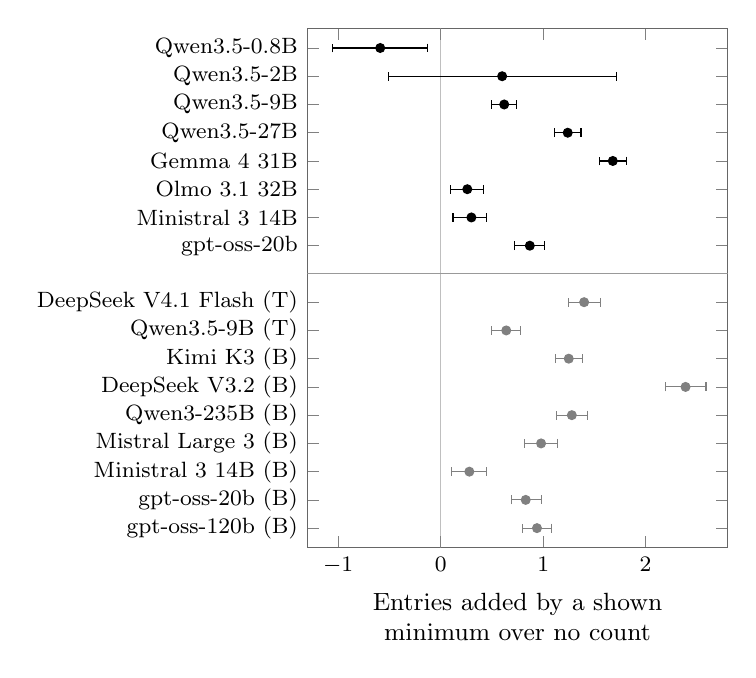
\begin{tikzpicture}
    \begin{axis}[scale only axis, width=0.44\columnwidth, height=6.6cm, xmin=-1.3, xmax=2.8,
                 xlabel={Entries added by a shown\\minimum over no count}, xlabel style={align=center},
                 padkCtwoTicks,
                 y tick label style={font=\footnotesize}, x tick label style={font=\footnotesize},
                 label style={font=\small}, ymin=0.3, ymax=18.7,
                 extra x ticks={0}, extra x tick style={grid=major, tick label style={opacity=0}},
                 axis line style={black!60}]
      \addplot[only marks, mark=*, mark size=1.6pt, color=black, mark options={fill=black}, error bars/.cd, x dir=both, x explicit] coordinates {
  (-0.59,18) -= (0.47,0) += (0.46,0)
  (0.60,17) -= (1.11,0) += (1.12,0)
  (0.62,16) -= (0.12,0) += (0.12,0)
  (1.24,15) -= (0.13,0) += (0.13,0)
  (1.68,14) -= (0.13,0) += (0.13,0)
  (0.26,13) -= (0.16,0) += (0.16,0)
  (0.30,12) -= (0.18,0) += (0.15,0)
  (0.87,11) -= (0.15,0) += (0.14,0)
};
\addplot[only marks, mark=*, mark size=1.6pt, color=gray, mark options={fill=gray}, error bars/.cd, x dir=both, x explicit] coordinates {
  (1.40,9) -= (0.15,0) += (0.16,0)
  (0.64,8) -= (0.14,0) += (0.14,0)
  (1.25,7) -= (0.13,0) += (0.13,0)
  (2.39,6) -= (0.20,0) += (0.20,0)
  (1.28,5) -= (0.15,0) += (0.15,0)
  (0.98,4) -= (0.16,0) += (0.16,0)
  (0.28,3) -= (0.17,0) += (0.17,0)
  (0.83,2) -= (0.14,0) += (0.15,0)
  (0.94,1) -= (0.14,0) += (0.14,0)
};

      \draw[black!40] (axis cs:-1.3,10) -- (axis cs:2.8,10);
    \end{axis}
  \end{tikzpicture}
  \caption{The main contrast per model: substantive entries under a \texttt{minItems} shown in the schema minus entries with no count, same document, documents with $n < k$, $k = 3$ and 5, with 95\% group-bootstrap intervals. Black: the eight GPU models. Grey, below the line: hosted reference models on Together (T) and Bedrock (B), never pooled with the GPU models.}
  \label{fig:headline}
\end{figure}

We find three things (Section~\ref{sec:results} marks which results are registered tests and which are exploratory or post hoc).

\textbf{Models treat the count as a target.}
A minimum shown in the schema, but not enforced, raises the share of lists longer than the true count from 34.5\% to 55.4\%: on the same documents, about one more list in five runs past the true count.
On the documents a model gets exactly right with no count, a shown minimum still makes about a third of its lists pad (35.2\%; post hoc).
Six of the eight GPU models and all nine hosted runs lengthen their lists; the exceptions are the two smallest models, one of which often writes no readable list (Section~\ref{sec:main}).
Registered controls tie the effect to the slots the document cannot fill: a minimum adds nothing on documents that already hold enough items, and a shown maximum barely changes over-count (Section~\ref{sec:named}).

\textbf{The padding is hard to catch.}
Most added entries are real text taken from the document, like the sign-off in Figure~\ref{fig:example}.
They parse, meet the schema, and about half pass a check that each entry occurs in the source (Section~\ref{sec:what}).

\textbf{Common fixes help only partly.}
A line saying fewer items are fine removes the effect on average but misses more true items.
An ``N/A'' option under an enforced minimum lowers padding only from 90.1\% to 51.0\%.
``Up to $k$'' in prose also raises over-counting, from 34.5\% to 42.7\%.
Re-asking with the bare validation error, as schema-validating libraries do, made padding far more common in every run tested, from 10.0\% to 69.0\% for Qwen3.5-9B (Section~\ref{sec:exploratory}).

Our contributions:
\begin{itemize}
  \setlength\itemsep{0pt}
  \item 558 real documents from nine annotated sets with answer lists checked by both authors, released with the code and run records (Section~\ref{sec:data}, Appendix~\ref{app:data}).
  \item A preregistered, per-model measurement of count pressure on eight open-weight models, with controls, and six hosted models as a reference (Section~\ref{sec:results}).
  \item Evidence that the padding is mostly real document text, with practical guidance for schema authors (Table~\ref{tab:guidance}).
\end{itemize}
